\index{Training}
\index{synthesis}
\index{neural network training}
\chapter{Training a Model from First Principles}
\printchapterversion{7_training_a_model}
\newthought{Oh, numerical methods are actually useful.}


% ==============================================================================================
% INTRODUCTION BLOCK

\section{The Why}
\index{training!motivation}


\newthought{The previous six chapters} developed numerical methdos.
These topics may appear distinct on a first reading,
but they share a wide-ranging application domain \cite{karpathy2019recipe}.


\index{chocolate}
\index{Nobel laureates}
\index{spurious correlation}

\newthought{The running dataset} for this chapter consists of fourteen countries with two associated quantities:
Per-capita chocolate consumption and Nobel laureates per ten million inhabitants \cite{messerlichocolate}.



\iffalse
\begin{table}[h]
\centering
\begin{tabular}{lrr}
\toprule
\textbf{Country} & \textbf{Chocolate} & \textbf{Nobel} \\
                 & (kg/person)        & (per 10M)      \\
\midrule
Switzerland    & 11.9 & 32 \\
Sweden         & 6.4  & 33 \\
Germany        & 11.6 & 13 \\
France         & 6.7  & 9  \\
United Kingdom & 9.5  & 21 \\
Norway         & 9.2  & 26 \\
Denmark        & 8.5  & 25 \\
Italy          & 4.0  & 4  \\
Netherlands    & 4.5  & 11 \\
Finland        & 7.3  & 7  \\
Austria        & 8.8  & 26 \\
Belgium        & 5.6  & 11 \\
United States  & 5.3  & 11 \\
Japan          & 1.8  & 2  \\
\bottomrule
\end{tabular}
\vspace{2em}
\caption{Per-capita chocolate consumption and Nobel laureates per ten million inhabitants.
Values are rounded and intended as a teaching dataset rather than as a research source.}
\label{tab:chocolate_data}
\end{table}
\fi


\newthought{The model} is a univariate linear regression of Nobel laureates on chocolate consumption (Figure~\ref{fig:chocolate_nobel_scatter}), fit by gradient descent on the mean squared error. The five correspondences below are illustrated against this model and dataset.


\begin{figure}[h]
    \centering
    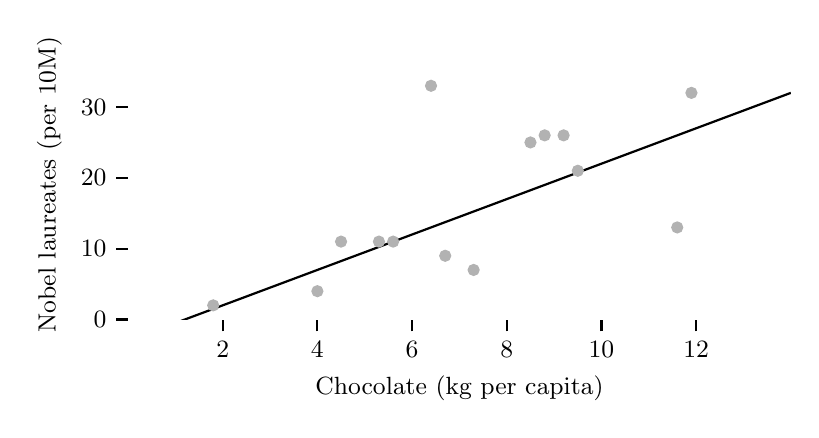
\begin{tikzpicture}
        \begin{axis}[
            width=10cm,
            height=5cm,
            xlabel={Chocolate (kg per capita)},
            ylabel={Nobel laureates (per 10M)},
            xmin=0, xmax=14,
            ymin=0, ymax=38,
            axis line style={draw=none},
            tick style={black, thick},
            xtick={2, 4, 6, 8, 10, 12},
            ytick={0, 10, 20, 30},
            xticklabel style={font=\small},
            yticklabel style={font=\small},
            tick align=outside,
            tick pos=left,
            label style={font=\small},
        ]
        \addplot[only marks, mark=*, mark size=2pt, gray!60] coordinates {
            (11.9, 32) (6.4, 33) (11.6, 13) (6.7, 9) (9.5, 21)
            (9.2, 26) (8.5, 25) (4.0, 4) (4.5, 11) (7.3, 7)
            (8.8, 26) (5.6, 11) (5.3, 11) (1.8, 2)
        };
        \addplot[black, thick, domain=0:14] {2.5*x - 3};
        \end{axis}
    \end{tikzpicture}
    \vspace{1em}
    \caption{The dataset and an approximate by-eye fit.
    The fit computed by gradient descent will not differ substantially.
    The Messerli correlation is real but spurious; chocolate consumption does not cause Nobel prizes, and plausible confounders include per-capita wealth and education.}
    \label{fig:chocolate_nobel_scatter}
\end{figure}


\marginnote{\newthought{Model}\\
$\hat{y}(x) = w x + b$.}

\marginnote{\newthought{Loss}\\
$L(w, b) = \tfrac{1}{n} \sum_{i=1}^{n} ( w x_i + b - y_i )^2$.}


\newthought{The Learning Objectives} are:
Identify numerical method in application, apply standard numerical methods in practical contexts, and finally think in frameworks.





% ==============================================================================================
% MAIN MIRRORS BLOCK

\newpage
\section{Overfitting as a Sanity Check}
\index{overfit single batch}
\index{Lagrange interpolation!model capacity}
\index{Newton method!sanity check}

\marginnote{\newthought{Recall Chapter 4.}
Newton's method converges in a single step from any starting point when applied to a quadratic function,
because the linear approximation of the derivative is exact in that case.}

\newthought{A standard recommendation in training} is to verify,
that the model can drive the loss to approximately zero on a small subset of the training data.
A failure to achieve this condition indicates an error in the model definition,
the loss formulation,
or the data pipeline.


\newthought{An example calculation} demonstrates the principle on a stripped down version of the dataset.
Pick just two countries, Italy at $(4.0, 4)$ and the United Kingdom at $(9.5, 21)$,
and extend the model by adding parameters,
\begin{align*}
    \hat{y}(x) = w_0 + w_1 x + w_2 x^2 + w_3 x^3 + w_4 x^4,
\end{align*}
with $n = 4$ here, giving five free parameters for only two training points.
The system is underdetermined:
infinitely many parameter settings drive the training loss to zero,
since any function passing through both training points qualifies.
A correctly implemented training loop on this overparameterized model must 
reach one of these zero-loss solutions (within machine precision).
Figure~\ref{fig:overfit_polynomial} shows one such solution:

\begin{figure}[h]
    \centering
    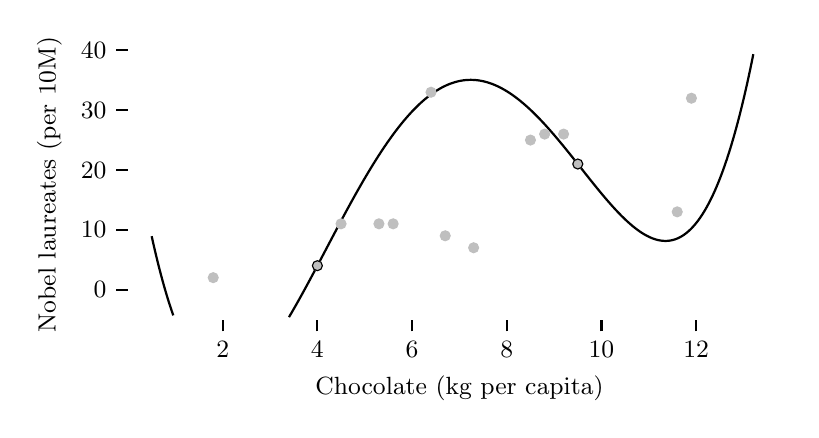
\begin{tikzpicture}
        \begin{axis}[
            width=10cm,
            height=5cm,
            xlabel={Chocolate (kg per capita)},
            ylabel={Nobel laureates (per 10M)},
            xmin=0, xmax=14,
            ymin=-5, ymax=40,
            restrict y to domain=-5:40,
            unbounded coords=jump,
            samples=400,
            axis line style={draw=none},
            tick style={black, thick},
            xtick={2, 4, 6, 8, 10, 12},
            ytick={0, 10, 20, 30, 40},
            xticklabel style={font=\small},
            yticklabel style={font=\small},
            tick align=outside,
            tick pos=left,
            label style={font=\small},
        ]
        \addplot[only marks, mark=*, mark size=1.8pt, gray!50] coordinates {
            (11.9, 32) (6.4, 33) (11.6, 13) (6.7, 9) (9.5, 21)
            (9.2, 26) (8.5, 25) (4.0, 4) (4.5, 11) (7.3, 7)
            (8.8, 26) (5.6, 11) (5.3, 11) (1.8, 2)
        };
        \addplot[black, thick, domain=0.5:13.5] {
            3.0909*x - 8.3636 + 0.08*(x-1)*(x-4)*(x-9.5)*(x-13)
        };
        \addplot[only marks, mark=o, mark size=1.8pt, black] coordinates {
            (4.0, 4) (9.5, 21)
        };
        \end{axis}
    \end{tikzpicture}
    \caption{Two training points (circled gray dots) selected from the dataset.
    Any function through both points is a zero-loss solution.
    It interpolates the two training points exactly but oscillates elsewhere,
    a textbook illustration of overfit capacity.}
    \label{fig:overfit_polynomial}
\end{figure}

\newthought{The sanity-check principle.}
The recommendation to drive the loss to zero on an overparameterized setup, where optimization is easy to achieve,
is the machine-learning instance of testing a solver on a problem with a known exact solution.

\vfill
\newthought{This separates the question of whether the implementation is correct
from the question of whether the method is suitable for the problem at hand.}

\marginnote{\newthought{Question.}
Figure~\ref{fig:overfit_polynomial} draws one zero-loss curve through the two training points.
How many such curves exist?
And what does that count imply about the geometry of the loss landscape this optimizer is asked to navigate? 
Welcome to the multiverse of global optima.}








\newpage
\section{Loss at Initialization}
\index{initialization!loss check}
\index{baseline test}

\marginnote{\newthought{Recall Chapter 4.}
A standard check for an iterative method, such as Newton's Method or SGD is to evaluate it at a configuration whose answer can be computed by hand.}

\newthought{A standard recommendation in training} is to inspect the loss before any optimization step has been taken.
The expected initial value follows from the data statistics and the chosen initialization;
a substantially different observed value points to a bug in the loss, the data, or the initialization.

\marginnote{\newthought{Classifier baseline.}
For a $K$-class classifier initialized to uniform output over the classes,
cross-entropy at step zero is $\log K$:
$\log 2 \approx 0.69$ for binary,
$\log 10 \approx 2.30$ for ten-way.
The first printed value is fixed by the architecture choice, not by the data.}

\newthought{An example calculation} on the chocolate dataset proceeds directly.
Initializing the regression with $w = 0$ and $b = \bar{y}$ makes the model predict $\bar{y}$ for every input,
so the mean squared error collapses to the mean squared deviation of the targets from their mean,
that is the empirical variance of the targets in the $1/n$ convention.
With $\bar{y} = 231/14 = 16.5$ and squared deviations summing to $1401.5$,
\begin{align*}
    L(0, \bar{y}) &= \frac{1}{n} \sum_{i=1}^{n} (y_i - \bar{y})^2 \\
                  &= \operatorname{Var}(y) \\
                  &\approx 100.1.
\end{align*}
A correct training loop therefore prints approximately $100$ as its first loss value.
A value of $5\,000$ indicates a summed rather than averaged loss;
a value of $0.0001$ indicates an unintended normalization;
a value far from $100$ in either direction indicates that the bias was not educatedly initialized (Figure~\ref{fig:init_loss}).


\begin{figure}[h]
    \centering
    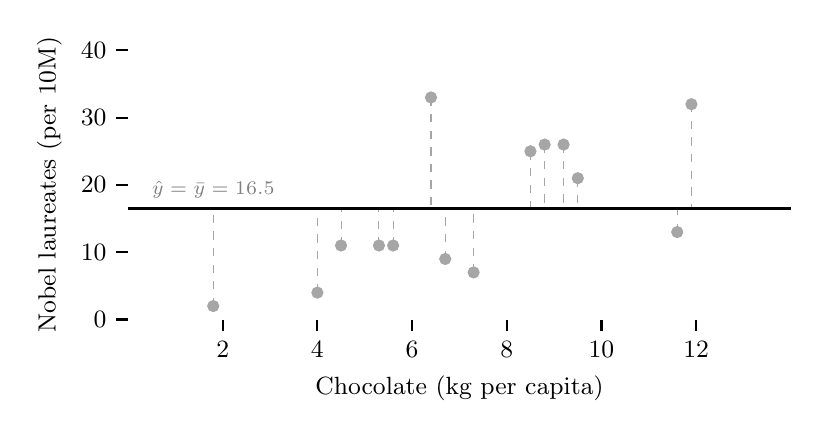
\begin{tikzpicture}
        \begin{axis}[
            width=10cm,
            height=5cm,
            xlabel={Chocolate (kg per capita)},
            ylabel={Nobel laureates (per 10M)},
            xmin=0, xmax=14,
            ymin=0, ymax=40,
            axis line style={draw=none},
            tick style={black, thick},
            xtick={2, 4, 6, 8, 10, 12},
            ytick={0, 10, 20, 30, 40},
            xticklabel style={font=\small},
            yticklabel style={font=\small},
            tick align=outside,
            tick pos=left,
            label style={font=\small},
        ]
        \addplot[gray!70, thin, dashed] coordinates {(1.8, 2) (1.8, 16.5)};
        \addplot[gray!70, thin, dashed] coordinates {(4.0, 4) (4.0, 16.5)};
        \addplot[gray!70, thin, dashed] coordinates {(4.5, 11) (4.5, 16.5)};
        \addplot[gray!70, thin, dashed] coordinates {(5.3, 11) (5.3, 16.5)};
        \addplot[gray!70, thin, dashed] coordinates {(5.6, 11) (5.6, 16.5)};
        \addplot[gray!70, thin, dashed] coordinates {(6.4, 33) (6.4, 16.5)};
        \addplot[gray!70, thin, dashed] coordinates {(6.7, 9) (6.7, 16.5)};
        \addplot[gray!70, thin, dashed] coordinates {(7.3, 7) (7.3, 16.5)};
        \addplot[gray!70, thin, dashed] coordinates {(8.5, 25) (8.5, 16.5)};
        \addplot[gray!70, thin, dashed] coordinates {(8.8, 26) (8.8, 16.5)};
        \addplot[gray!70, thin, dashed] coordinates {(9.2, 26) (9.2, 16.5)};
        \addplot[gray!70, thin, dashed] coordinates {(9.5, 21) (9.5, 16.5)};
        \addplot[gray!70, thin, dashed] coordinates {(11.6, 13) (11.6, 16.5)};
        \addplot[gray!70, thin, dashed] coordinates {(11.9, 32) (11.9, 16.5)};
        \addplot[black, thick, domain=0:14] {16.5};
        \addplot[only marks, mark=*, mark size=2pt, gray!70] coordinates {
            (11.9, 32) (6.4, 33) (11.6, 13) (6.7, 9) (9.5, 21)
            (9.2, 26) (8.5, 25) (4.0, 4) (4.5, 11) (7.3, 7)
            (8.8, 26) (5.6, 11) (5.3, 11) (1.8, 2)
        };
        \node[anchor=south west, font=\scriptsize, text=gray] at (axis cs:0.3, 16.5) {$\hat{y} = \bar{y} = 16.5$};
        \end{axis}
    \end{tikzpicture}
    \caption{Initialization with $w = 0$ and $b = \bar{y}$ predicts the constant $\bar{y} = 16.5$ for every input (horizontal line).
    The vertical segments are the residuals $y_i - \bar{y}$;
    the mean of their squares is the initial loss, $\operatorname{Var}(y) \approx 100$.}
    \label{fig:init_loss}
\end{figure}


\newthought{The boundary-value principle.}
A hand-computable value at a known starting configuration is the universal first verification step for any numerical procedure;
inspecting the initial loss against the variance of the targets is one instance.
It separates a failure of implementation, visible at step zero, from a failure of optimization, which can only show up after the first step is taken.






\newpage
\section{Mini-Batch Stochastic Gradient Descent}
\index{stochastic gradient descent}
\index{Monte Carlo!gradient}

\marginnote{\newthought{Curse of Dimensionality}
Monte Carlo integration averages the integrand at random samples and has standard error $1/\sqrt{N}$ independently of the dimension of the domain.
That dimension independence is what distinguishes it from grid quadrature, whose cost grows exponentially.}


\newthought{There is sample $x_n$ and feature dimension $d$,} use mini-batch stochastic gradient descent in place of 
full-batch gradient descent when dealing with data at scale.
At each iteration the gradient is estimated from a small random subset 
of the training data rather than from the entire dataset.
The loss is an expectation,
\begin{align*}
    L(\theta) = \mathbb{E}_{x \sim p_{\text{data}}} \big[ \ell(x; \theta) \big],
\end{align*}
and so is its gradient.
This substitution is not new.
The secant method in Chapter 4 replaced the exact derivative with a two-point finite-difference estimate,
and Newton's method replaced the objective with a truncated Taylor expansion.
Mini-batch stochastic gradient descent applies the same pattern on the data axis.

\newthought{An example calculation} on the chocolate dataset makes the variance visible.
Two mini-batches of size $B = 2$ are drawn from the fourteen countries; each yields the line through its two points,
\begin{align*}
    \hat{y}_P &= 3.54 x - 10.18, \\
    \hat{y}_Q &= -1.43 x + 17.43.
\end{align*}
The approximated gradient is the delta between the mini-batch line and the current overall approximation,
so each mini-batch supplies its own estimate of the same update direction,
and the spread of those deltas quantifies the variance of the stochastic estimator.

\begin{figure}[h]
    \centering
    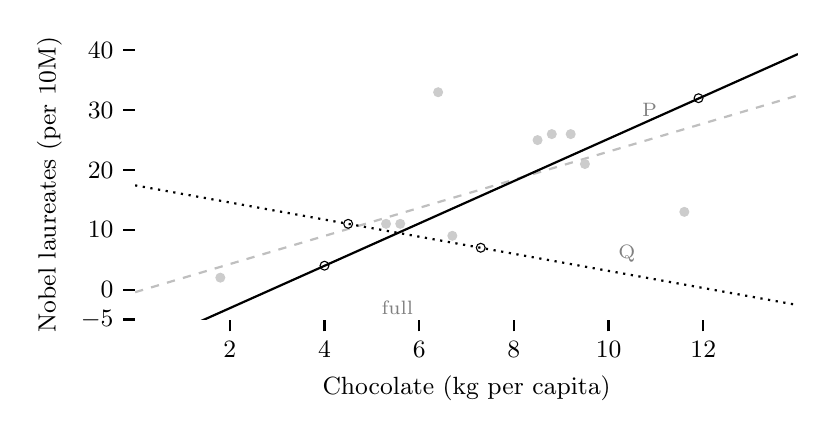
\begin{tikzpicture}
        \begin{axis}[
            width=10cm,
            height=5cm,
            xlabel={Chocolate (kg per capita)},
            ylabel={Nobel laureates (per 10M)},
            xmin=0, xmax=14,
            ymin=-5, ymax=40,
            axis line style={draw=none},
            tick style={black, thick},
            xtick={2, 4, 6, 8, 10, 12},
            ytick={-5, 0, 10, 20, 30, 40},
            xticklabel style={font=\small},
            yticklabel style={font=\small},
            tick align=outside,
            tick pos=left,
            label style={font=\small},
        ]
        % Full-batch reference fit
        \addplot[gray!50, thick, dashed, domain=0:14] {2.35*x - 0.43};
        % Mini-batch fits
        \addplot[black, thick, domain=0:14] {3.54*x - 10.18};
        \addplot[black, thick, dotted, domain=0:14] {-1.43*x + 17.43};
        % Unused data points (grayed out)
        \addplot[only marks, mark=*, mark size=1.6pt, gray!40] coordinates {
            (6.4, 33) (11.6, 13) (6.7, 9) (9.5, 21) (9.2, 26)
            (8.5, 25) (8.8, 26) (5.6, 11) (5.3, 11) (1.8, 2)
        };
        % Mini-batch A points (used for solid fit)
        \addplot[only marks, mark=o, mark size=1.6pt, black] coordinates {
            (4.0, 4) (11.9, 32)
        };
        % Mini-batch B points (used for dotted fit)
        \addplot[only marks, mark=o, mark size=1.6pt, black] coordinates {
            (4.5, 11) (7.3, 7)
        };
        \node[anchor=west, font=\scriptsize, text=gray] at (axis cs:10.5, 30) {P};
        \node[anchor=west, font=\scriptsize, text=gray] at (axis cs:10, 6) {Q};
        \node[anchor=west, font=\scriptsize, text=gray] at (axis cs:5, -3) {full};
        \end{axis}
    \end{tikzpicture}
    \caption{Two mini-batch fits to the chocolate dataset,
    each passing through its two sampled countries (P solid, Q dotted),
    together with the current overall approximation (gray dashed).
    Open circles mark the points used by each fit; the remaining countries are grayed out.
    The approximated gradient is the delta between a mini-batch line and the current overall approximation.}
    \label{fig:minibatch_estimates}
\end{figure}

\vfill
\newthought{The stochastic-gradient principle.}
Mini-batch SGD is a moving target per step but not in expectation:
iterates fluctuate in a neighborhood of the minimum whose radius shrinks with the step size and with the batch.
The same noise that bars exact convergence dislodges iterates from shallow local minima where full-batch descent would settle.



\marginnote{\newthought{Question.}
For $n = 14$ a batch of $B = 4$ buys nothing; for $n = 10^9$ the full batch never fits in memory.
At which $n$ does the bottleneck flip with $1/\sqrt{B}$?}





\iffalse
\newpage
\section{The Shape of the Loss Curve}
\index{loss curve}
\index{conditioning!loss curve}
\index{neural network!loss landscape}

\marginnote{\newthought{Recall Chapter 3.}
The convergence rate of gradient descent on a quadratic loss is governed by the condition number $\kappa$.
The error after $n$ iterations contracts by a factor $\bigl((\kappa-1)/(\kappa+1)\bigr)^n$,
so small $\kappa$ converges rapidly and large $\kappa$ crawls.}

\newthought{A standard recommendation in training} is attentive inspection of the loss curve throughout the run.
The shape of the curve, not its final value alone, carries the diagnostic content.

\newthought{An example calculation} on the chocolate dataset makes the link concrete.
With a single normalized feature, the condition number is small, perhaps $\kappa \approx 5$,
and the contraction factor is
\begin{align*}
    \frac{\kappa - 1}{\kappa + 1} = \frac{4}{6} \approx 0.67,
\end{align*}
so each iteration shrinks the error to about two thirds of its previous value and the curve settles within a handful of steps.
Adding a second feature without rescaling, for instance per-capita GDP in single euros, sends $\kappa$ to the order of $10^{10}$, the contraction factor to essentially one, and the loss curve to apparent flatness for any practical duration of training.
Figure~\ref{fig:loss_curve_shape} contrasts the two regimes on a common axis.

\begin{figure}[h]
    \centering
    \begin{tikzpicture}
        \begin{axis}[
            width=10cm,
            height=5cm,
            xlabel={iteration $n$},
            ylabel={loss $L_n$},
            xmin=0, xmax=50,
            ymin=0.01, ymax=100,
            ymode=log,
            log basis y=10,
            axis line style={draw=none},
            tick style={black, thick},
            xtick={0, 10, 20, 30, 40, 50},
            ytick={0.01, 0.1, 1, 10, 100},
            xticklabel style={font=\small},
            yticklabel style={font=\small},
            tick align=outside,
            tick pos=left,
            label style={font=\small},
        ]
        \addplot[black, thick, samples=51, domain=0:50]
            {100 * ((5-1)/(5+1))^x};
        \addplot[black, thick, dashed, samples=51, domain=0:50]
            {100 * ((100-1)/(100+1))^x};
        \node[anchor=west, font=\scriptsize, text=gray] at (axis cs:11, 0.5) {$\kappa{=}5$};
        \node[anchor=west, font=\scriptsize, text=gray] at (axis cs:30, 40) {$\kappa{=}100$};
        \end{axis}
    \end{tikzpicture}
    \caption{Loss curves of gradient descent on the chocolate dataset under two conditioning regimes,
    log scale on the loss axis.
    The solid curve corresponds to a well-conditioned setup ($\kappa = 5$) and reaches near-zero loss within a handful of iterations.
    The dashed curve corresponds to an ill-conditioned setup ($\kappa = 100$) and crawls.
    The shape of the curve identifies the regime.}
    \label{fig:loss_curve_shape}
\end{figure}

\newthought{Neural networks complicate the picture but reuse the instinct.}
The high-dimensional non-convex landscape of a deep network has mostly saddle points rather than minima \cite{DeepLearningBookNumericalComputation},
so a long plateau may signal an ill-conditioned quadratic or a slow escape from a saddle, and a sharp drop may signal a cliff.
The vocabulary expands; reading the curve as the first diagnostic does not.

\newthought{The conditioning principle.}
The recommendation to read the loss curve and the numerical methods practice of inferring the condition number from a convergence rate are the same procedure.

\vfill
\newthought{This reuses one diagnostic instinct} across convex regression and non-convex deep learning alike.

\marginnote{\newthought{Question.}
If your loss curve is flat for one hundred steps, is your problem ill-conditioned, stuck at a saddle, or just plain broken?
And how would you tell the three apart with one more experiment?
The curve talks; the question is whether you listen.}




\newpage
\section{Random Hyperparameter Search}
\index{hyperparameter search}
\index{curse of dimensionality}
\index{Monte Carlo!hyperparameters}

\marginnote{\newthought{Recall Chapter 6.}
In a $d$-dimensional cube, a grid with $N$ points per axis requires $N^d$ evaluations.
Monte Carlo accuracy depends on the total number of samples, not on $d$,
so for any but the smallest $d$ random sampling outperforms grid evaluation.}

\newthought{Standard practice} is to tune hyperparameters by random sampling of the hyperparameter space rather than by exhaustive grid search.
Random search consistently finds better configurations within a given compute budget;
a grid search that still terminates on a non-trivial model signals either a very small search space or a misallocated budget.

\newthought{An example calculation} makes the cost comparison concrete.
Tuning $d$ hyperparameters with $N = 5$ values per axis costs $N^d = 5^d$ evaluations by grid:
five at $d = 1$, three thousand at $d = 5$, nearly ten million at $d = 10$.
The random-search budget required for a fixed target accuracy is constant in $d$, by the dimension independence of Monte Carlo.
Figure~\ref{fig:curse_hyperparam} contrasts the two curves on a log axis.

\begin{figure}[h]
    \centering
    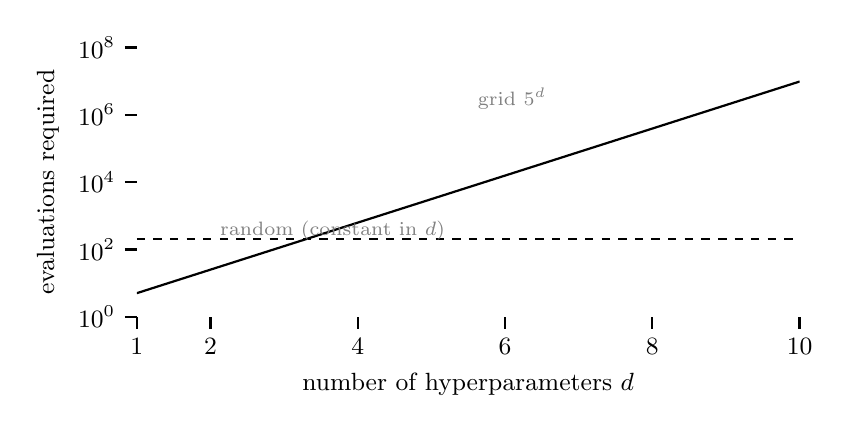
\begin{tikzpicture}
        \begin{axis}[
            width=10cm,
            height=5cm,
            xlabel={number of hyperparameters $d$},
            ylabel={evaluations required},
            xmin=1, xmax=10,
            ymin=1, ymax=1e8,
            ymode=log,
            log basis y=10,
            axis line style={draw=none},
            tick style={black, thick},
            xtick={1, 2, 4, 6, 8, 10},
            ytick={1, 100, 10000, 1000000, 100000000},
            xticklabel style={font=\small},
            yticklabel style={font=\small},
            tick align=outside,
            tick pos=left,
            label style={font=\small},
        ]
        \addplot[black, thick, samples=10, domain=1:10] {5^x};
        \addplot[black, thick, dashed, samples=10, domain=1:10] {200};
        \node[anchor=west, font=\scriptsize, text=gray] at (axis cs:5.5, 3e6) {grid $5^d$};
        \node[anchor=west, font=\scriptsize, text=gray] at (axis cs:2, 350) {random (constant in $d$)};
        \end{axis}
    \end{tikzpicture}
    \caption{Evaluations required by grid search ($5^d$) versus random sampling for a fixed target accuracy,
    on log axes.
    The grid cost grows exponentially with $d$;
    the random-search budget does not.
    For more than a handful of hyperparameters,
    only the latter is realistic.}
    \label{fig:curse_hyperparam}
\end{figure}

\newthought{The dimension-independence principle.}
Mini-batch stochastic gradient descent applies Monte Carlo to the gradient integral;
random hyperparameter search applies Monte Carlo to the validation-loss landscape.
Both rely on the same property: accuracy that does not depend on $d$.

\vfill
\newthought{This reuses the same square-root bound} that justified mini-batch training one section ago, in a different ambient dimension.

\marginnote{\newthought{Question.}
You have a budget of two hundred runs and seven hyperparameters to tune.
Where does a grid land you, where does random search land you, and how many of those seven are you secretly hoping do not matter?
Choose your dimensions before they choose you.}


\fi

\newpage
\section{Training Multiple Random Seeds}
% TODO find a better function to showcase this.. also a local minima would be nice, so we see two curves in the marginnote figure.
% Uncommented because like this it is not really worth it.
\index{global optimization}
\index{random restarts}

\marginnote{\newthought{Recall Chapter 5.}
For a non-convex objective, gradient descent terminates at a local minimum that depends on the initial point.
An effective global-optimization strategy is random restarts.}

\newthought{Repeat} training from several random initializations 
of the model parameters. The variance across runs is diagnostic about the loss landscape, 
and the run with the lowest loss is the candidate global solution \cite{picard2021seed}. 

\newthought{Composing} the slope from two parameters, with a quadratic trick on $w$ to 
introduce a symmetry, gives a concrete example of the principle.
\begin{align*}
    \hat{y}(x) = w^2 x + b.
\end{align*}
with minima at $w \approx \pm 1.53$ ($L \approx 60$) and a saddle at $w = 0$ ($L \approx 100$).

\marginnote{\newthought{Which would not have hurt at all} to be fair.} 

\newthought{With} two random starts, shown as circles in Figure~\ref{fig:multiple_seeds}.
Both basins recover the same fit $\hat{y} = 2.34 x - 0.43$;
a single seed would have surfaced only one solution in the whole space.

\vspace{1.5em}



\begin{figure}[h]
    \centering
    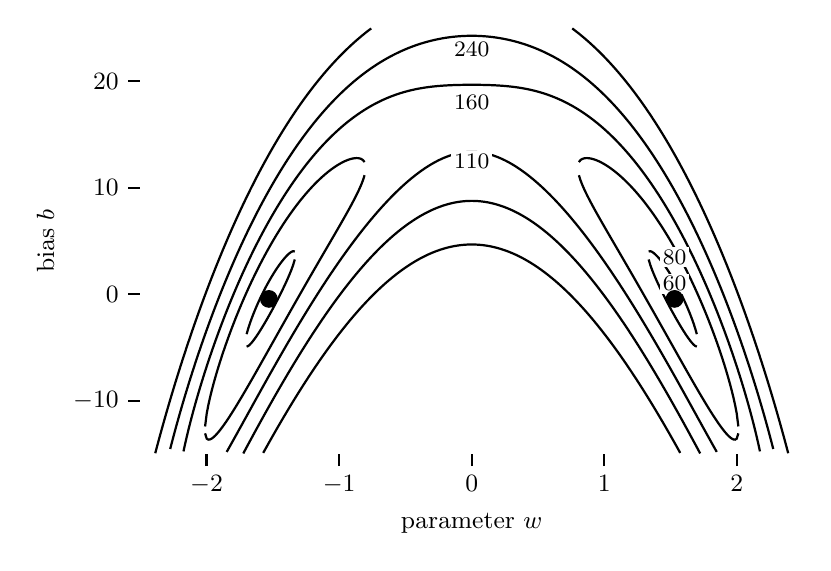
\begin{tikzpicture}
        \begin{axis}[
            width=10cm,
            height=7cm,
            xlabel={parameter $w$},
            ylabel={bias $b$},
            xmin=-2.5, xmax=2.5,
            ymin=-15, ymax=25,
            restrict y to domain=-15:25,
            unbounded coords=jump,
            axis line style={draw=none},
            tick style={black, thick},
            xtick={-2, -1, 0, 1, 2},
            ytick={-10, 0, 10, 20},
            xticklabel style={font=\small},
            yticklabel style={font=\small},
            tick align=outside,
            tick pos=left,
            label style={font=\small},
        ]
        \addplot[domain=-2.5:2.5, samples=400, thick, black]
          {(60 - 7.773*x^4 + 36.44*x^2 - 100.107 > 0) ? 16.5 - 7.221*x^2 + sqrt(60 - 7.773*x^4 + 36.44*x^2 - 100.107) : 1000};
        \addplot[domain=-2.5:2.5, samples=400, thick, black]
          {(60 - 7.773*x^4 + 36.44*x^2 - 100.107 > 0) ? 16.5 - 7.221*x^2 - sqrt(60 - 7.773*x^4 + 36.44*x^2 - 100.107) : 1000};
        \addplot[domain=-2.5:2.5, samples=400, thick, black]
          {(80 - 7.773*x^4 + 36.44*x^2 - 100.107 > 0) ? 16.5 - 7.221*x^2 + sqrt(80 - 7.773*x^4 + 36.44*x^2 - 100.107) : 1000};
        \addplot[domain=-2.5:2.5, samples=400, thick, black]
          {(80 - 7.773*x^4 + 36.44*x^2 - 100.107 > 0) ? 16.5 - 7.221*x^2 - sqrt(80 - 7.773*x^4 + 36.44*x^2 - 100.107) : 1000};
        \addplot[domain=-2.5:2.5, samples=400, thick, black]
          {(110 - 7.773*x^4 + 36.44*x^2 - 100.107 > 0) ? 16.5 - 7.221*x^2 + sqrt(110 - 7.773*x^4 + 36.44*x^2 - 100.107) : 1000};
        \addplot[domain=-2.5:2.5, samples=400, thick, black]
          {(110 - 7.773*x^4 + 36.44*x^2 - 100.107 > 0) ? 16.5 - 7.221*x^2 - sqrt(110 - 7.773*x^4 + 36.44*x^2 - 100.107) : 1000};
        \addplot[domain=-2.5:2.5, samples=400, thick, black]
          {(160 - 7.773*x^4 + 36.44*x^2 - 100.107 > 0) ? 16.5 - 7.221*x^2 + sqrt(160 - 7.773*x^4 + 36.44*x^2 - 100.107) : 1000};
        \addplot[domain=-2.5:2.5, samples=400, thick, black]
          {(160 - 7.773*x^4 + 36.44*x^2 - 100.107 > 0) ? 16.5 - 7.221*x^2 - sqrt(160 - 7.773*x^4 + 36.44*x^2 - 100.107) : 1000};
        \addplot[domain=-2.5:2.5, samples=400, thick, black]
          {(240 - 7.773*x^4 + 36.44*x^2 - 100.107 > 0) ? 16.5 - 7.221*x^2 + sqrt(240 - 7.773*x^4 + 36.44*x^2 - 100.107) : 1000};
        \addplot[domain=-2.5:2.5, samples=400, thick, black]
          {(240 - 7.773*x^4 + 36.44*x^2 - 100.107 > 0) ? 16.5 - 7.221*x^2 - sqrt(240 - 7.773*x^4 + 36.44*x^2 - 100.107) : 1000};
        \node[font=\footnotesize, fill=white, inner sep=1pt] at (axis cs:1.53, 1.0) {60};
        \node[font=\footnotesize, fill=white, inner sep=1pt] at (axis cs:1.53, 3.5) {80};
        \node[font=\footnotesize, fill=white, inner sep=1pt] at (axis cs:0, 12.5) {110};
        \node[font=\footnotesize, fill=white, inner sep=1pt] at (axis cs:0, 18) {160};
        \node[font=\footnotesize, fill=white, inner sep=1pt] at (axis cs:0, 23) {240};
        \addplot[only marks, mark=*, mark size=3pt, black]
            coordinates {(-1.53, -0.43) (1.53, -0.43)};
        \end{axis}
    \end{tikzpicture}
    \caption{Loss landscape $L(w, b)$ for $\hat{y}(x) = w^2 x + b$ on the chocolate data, drawn as iso-loss contours.
    Filled circles mark the two converged minima at $(w, b) = (\pm 1.53, -0.43)$ with $L \approx 57.4$,
    sitting on the curved valley $b^*(w) = 16.5 - 7.221\, w^2$. My wife also says it looks like the whale from 
    "Hitchhiker's Guide to the Galaxy". Okay, I added the book reference.}
    \label{fig:multiple_seeds}
\end{figure}

\iffalse
\begin{marginfigure}
    \centering
    \begin{tikzpicture}
        \begin{axis}[
            width=\marginparwidth,
            height=4cm,
            xlabel={Chocolate},
            ylabel={Nobel},
            xmin=0, xmax=14,
            ymin=0, ymax=38,
            axis line style={draw=none},
            tick style={black, thick},
            xtick={2, 6, 10},
            ytick={10, 20, 30},
            xticklabel style={font=\footnotesize},
            yticklabel style={font=\footnotesize},
            tick align=outside,
            tick pos=left,
            label style={font=\footnotesize},
        ]
        \addplot[only marks, mark=*, mark size=1.5pt, gray!60] coordinates {
            (11.9, 32) (6.4, 33) (11.6, 13) (6.7, 9) (9.5, 21)
            (9.2, 26) (8.5, 25) (4.0, 4) (4.5, 11) (7.3, 7)
            (8.8, 26) (5.6, 11) (5.3, 11) (1.8, 2)
        };
        \addplot[black, thick, domain=0:14] {1.53^2 * x - 0.43};
        \end{axis}
    \end{tikzpicture}
    \caption{Both minima of Figure~\ref{fig:multiple_seeds} produce the same fit $\hat{y} = 2.34\,x - 0.43$ on the chocolate data, since $w^2$ erases the sign of $w$.}
    \label{fig:multiple_seeds_fit}
\end{marginfigure}
\fi

\newthought{Cost Benefits}. Purely tuning the learning rate to chase variance that is actually 
basin-selection variance, is a common failure mode.

\newthought{Cost caveat.}
Multi-seed training multiplies compute by the number of seeds.
Routine at small-scale; at scale
the method only survives in partial-data form.
However, an empirical observation shows that,
distinct trained minima are typically joined by low-loss paths in parameter space as model-scale grows 
\cite{garipov2018modeconnectivity}.









\newpage
\section{Quantization for Inference}
\index{quantization}
\index{binary precision}

\marginnote{\newthought{Recall Chapter 2.}
Floating-point formats trade range against precision against bits.
The appropriate format for a given computation is the smallest one whose range and precision suffice.}

\newthought{The savings fall in two areas.}
At training time, parameters and gradients move less data through memory;
per-step throughput on bandwidth-bound hardware rises in proportion,
and even when low precision demands more steps to reach a comparable loss the product, 
operations until convergence, often remains favourable.
At inference the win compounds: floating-point multiplications collapse into cheap bitwise operations on dedicated hardware,
and a model whose parameters fit in cache stops paying the memory-latency tax that dominates inference for anything larger than the L2.

\begin{marginfigure}
    \centering
    \begin{tikzpicture}
        \begin{axis}[
            width=\marginparwidth,
            height=4cm,
            xlabel={bits per parameter},
            ylabel={loss},
            xmode=log,
            log basis x={2},
            xmin=0.7, xmax=45,
            ymin=6, ymax=15,
            axis line style={draw=none},
            tick style={black, thick},
            xtick={1, 8, 32},
            xticklabels={1, 8, 32},
            ytick={8, 10, 12, 14},
            xticklabel style={font=\footnotesize},
            yticklabel style={font=\footnotesize},
            tick align=outside,
            tick pos=left,
            label style={font=\footnotesize},
        ]
        \addplot[black, thick, mark=*, mark size=1.8pt] coordinates {
            (1, 13.3) (8, 7.9) (32, 7.6)
        };
        \end{axis}
    \end{tikzpicture}
    \caption{Loss against bits per parameter on the chocolate dataset.
    Binary precision pays a sharp penalty; the curve drops fast and flattens by integer precision.
    Most of the win sits in the first few bits.}
    \label{fig:precision_loss}
\end{marginfigure}

\newthought{An example calculation} on the chocolate model makes the trade visible.
Full-precision fitting, integer rounding to the nearest integer, and binary rounding 
to the nearest representative in $\{-1, +1\}$ produce three lines,
\begin{align*}
    &\hat{y}_{\text{full}}   = 2.35 x - 0.43, \\
    &\hat{y}_{\text{int}}    = 2 x, \\
    &\hat{y}_{\text{binary}} = x - 1.
\end{align*}
with root-mean-square errors
\begin{align*}
    &\text{L}_{\text{full}}   \approx 7.6, \\
    &\text{L}_{\text{int}}    \approx 7.9, \\
    &\text{L}_{\text{binary}} \approx 13.3,
\end{align*}




measured in Nobel laureates per ten million.
Figure~\ref{fig:binary_fit} overlays the three on the dataset.


\begin{figure}[h]
    \centering
    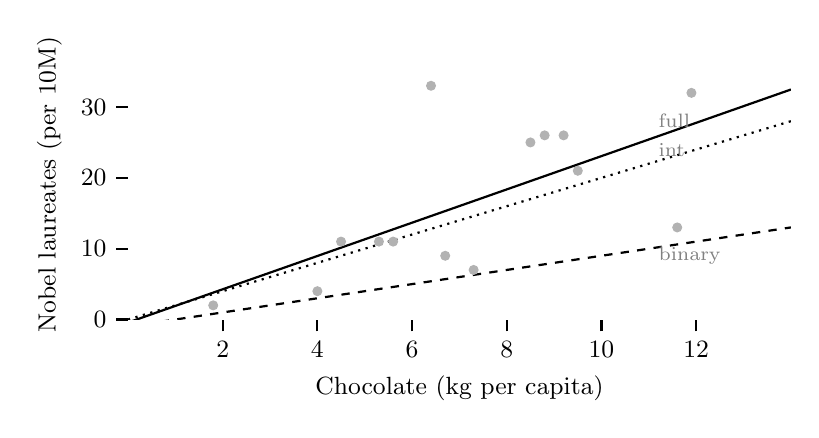
\begin{tikzpicture}
        \begin{axis}[
            width=10cm,
            height=5cm,
            xlabel={Chocolate (kg per capita)},
            ylabel={Nobel laureates (per 10M)},
            xmin=0, xmax=14,
            ymin=0, ymax=38,
            axis line style={draw=none},
            tick style={black, thick},
            xtick={2, 4, 6, 8, 10, 12},
            ytick={0, 10, 20, 30},
            xticklabel style={font=\small},
            yticklabel style={font=\small},
            tick align=outside,
            tick pos=left,
            label style={font=\small},
        ]
        \addplot[only marks, mark=*, mark size=1.6pt, gray!60] coordinates {
            (11.9, 32) (6.4, 33) (11.6, 13) (6.7, 9) (9.5, 21)
            (9.2, 26) (8.5, 25) (4.0, 4) (4.5, 11) (7.3, 7)
            (8.8, 26) (5.6, 11) (5.3, 11) (1.8, 2)
        };
        \addplot[black, thick, domain=0:14] {2.35*x - 0.43};
        \addplot[black, thick, dotted, domain=0:14] {2*x};
        \addplot[black, thick, dashed, domain=0:14] {x - 1};
        \node[anchor=west, font=\scriptsize, text=gray] at (axis cs:11, 28) {full};
        \node[anchor=west, font=\scriptsize, text=gray] at (axis cs:11, 24) {int};
        \node[anchor=west, font=\scriptsize, text=gray] at (axis cs:11, 9) {binary};
        \end{axis}
    \end{tikzpicture}
    \caption{Full-precision fit (solid), integer approximation $(w, b) = (2, 0)$ (dotted), and binary approximation $(w, b) = (+1, -1)$ (dashed) on the chocolate dataset.
    Integer rounding barely moves the root-mean-square error; binary near doubles it.}
    \label{fig:binary_fit}
\end{figure}


\vfill
\newthought{And another tradeoff,} where we give up precision and predictive performacnce, for runtime, memory and energy savings.

\marginnote{\newthought{Question.}
Integer precision matched the full-precision error on this dataset.
Why does any production model still ship in float32?
Where does the extra precision actually earn its bits, and where is it just inertia?}




% ==============================================================================================
% STUDENT ACTIVATION + RECAP BLOCK

\newpage
\section{Self-Reflection and Recap}
\index{recap}
\index{reflection}

\newthought{Self-Reflection} Questions to guide your understanding:
\begin{itemize}
    \item Why does driving the loss to zero on an overparameterized model detect bugs in the pipeline rather than in the optimizer?
    \item For the chocolate model initialized at $w = 0$, $b = \bar{y}$, the predicted first loss is $\operatorname{Var}(y) \approx 100$. What does a printed value of $5\,000$ tell you, and what does a printed value of $0.0001$ tell you?
    \item In what precise sense is mini-batch stochastic gradient descent a Monte Carlo estimator? What is being averaged, and over what?
    \item For the factored model $\hat{y}(x) = w^2 x + b$, why is the origin a saddle of the loss rather than a minimum, and what makes zero initialization a practical trap even so?
    \item Why can a model trained at higher precision be deployed at much lower precision without retraining, while training at the lower precision tends to fail?
\end{itemize}

\newthought{Recap} of Key Concepts:
\begin{itemize}
    \item Driving the loss to zero on an overparameterized model is the training version of testing a solver on a problem with a known exact answer.
    \item Inspecting the initial loss against the variance of the targets separates a failure of implementation, visible at step zero, from a failure of optimization, which can only appear after the first step.
    \item Mini-batch stochastic gradient descent is Monte Carlo applied to the gradient integral, with standard error $1/\sqrt{B}$ independent of the parameter dimension.
    \item Training from multiple random seeds is the random-restarts heuristic from Chapter 5 applied to a non-convex landscape; the seed picks the basin through the sign of the initial fluctuation at the origin saddle, and mini-batch noise supplies the annealing component implicitly.
    \item Quantization for inference is the precision-selection decision from Chapter 2 applied to a different computation: inference tolerates far less precision than training because it does not accumulate gradient updates, so the appropriate format is the smallest whose error budget is acceptable for the deployment.
\end{itemize}

\marginnote[2em]{\newthought{Outlook.} The same numerical methods (often) scale to billion-parameter models.
The cost and the engineering grow; the methods do not.}

\newthought{From numerical methods to modeling at scale.} The toolbox established in Chapters 1 to 6
is sufficient to describe the standard practices of model training at the scale of these notes.
At larger scales the parameter count grows by orders of magnitude and the data, too.
The engineering surrounding the training run grows correspondingly,
and the vocabulary drifts further from the language of classical numerical analysis.
None of this displaces the underlying methods.
The mechanics that decide whether a model's learning succeeds remain those introduced earlier.



% ==============================================================================================
% POTENTIAL ADD-ON MIRRORS (for future expansion; not currently in chapter)
%
% Each entry: Recipe recommendation  ↔  Corresponding numerical method (chapter)
% These correspondences were considered but not included, either because they
% require introducing material not yet covered in Chapters 1 to 6, or because
% they would lengthen the chapter past one correspondence per page.
%
% - Input-independent baseline (third Karpathy sanity-check step)
%       ↔ Degenerate input test for a numerical procedure (Ch3 + Ch6, quadrature
%         on a constant function should return constant times interval, etc.)
%
% - Weight decay
%       ↔ Tikhonov regularization for ill-conditioned inverse problems (Ch3,
%         would require introducing Tikhonov first)
%
% - Learning-rate schedules (cosine, warmup)
%       ↔ Adaptive step-size in iterative methods (Ch5, would need step-size
%         control as a new concept)
%
% - Adam and momentum-based optimizers
%       ↔ Heavy-ball and second-order methods (Ch4/Ch5, would need momentum
%         as a new concept)
%
% - Batch normalization
%       ↔ Per-layer preconditioning (Ch3, would need the depth-composition
%         argument that the chapter currently avoids)
%
% - Dropout
%       ↔ Random projection or ensemble of subsets (Ch6, would need a new
%         framing of dropout as Monte Carlo over sub-networks)
%
% - Early stopping
%       ↔ Truncation of an iterative method before machine precision is hit
%         (Ch4/Ch5, conceptually direct but pedagogically thin)
%
% - Gradient checkpointing
%       ↔ Space-time tradeoff in numerical computation (would need a separate
%         treatment of memory-compute tradeoffs)
%
% - Initial use of a default optimizer such as Adam
%       ↔ Use of the simplest sufficient method as a first choice (Ch5,
%         pedagogically thin)
%
% - Data augmentation
%       ↔ Importance sampling and variance reduction in Monte Carlo (Ch6,
%         would need importance sampling introduced first)
%
% - Mixed-precision training with loss scaling
%       ↔ Affine rescaling to keep values within the representable range
%         (Ch2, conceptually direct but adds a second Ch2 correspondence
%         beyond Correspondence 7)
%
% - Curriculum learning, easy-to-hard training
%       ↔ Homotopy and continuation methods in nonlinear solvers (would need
%         continuation as a new concept)
%
% ==============================================================================================

%%%%%%%%%%%%%%%%%%%%%%%%%%%%%%%%%%%%%%%%%%%%%%%%%%%%%%%%%%%%%%%%%%%%%%%%%%%%%%
